\section{QoI Model}
\label{sec:qoi_model}

Let us define the following terms:

\begin{itemize}
  \item $W$ = Channel Rate (bits/second)
  \item $T$ = Timeliness Requirement (seconds)
  \item $k_{req}$ = Number of required images
  \item $I_S$ = Size of each image (bits)
  \item $CF$ = Channel Factor
  \item $TF$ = Traffic Factor
  \item $P_S$ = Packet size
  \item $DF$ = Delay Factor
  \item $PL$ = Path Length
\end{itemize}

In the DCOSS submission we derived the following equation for scalability that uses each of these defined terms:
\begin{equation}
	W \cdot T - k_{req} \cdot I_S \cdot CF \cdot TF - P_S \cdot DF \cdot (PL-1) \geq 0	
\end{equation}

If we rearrange this equation, we can view the satisfiability of timeliness in terms of delay components:
\begin{equation}
	T \geq \frac{ k_{req} \cdot I_S \cdot CF \cdot TF}{W} + \frac{P_S \cdot DF \cdot (PL-1)}{W}
\end{equation}

In our previous analysis, we strive to determine the limits of this timeliness satisfiability by utilizing some static values and some average values where appropriate in this relation.  The resulting analysis provided approximate values for QoI satisfiability and network scalability, but what if we want to expand satisfiability to a stochastic definition?  And/or can we provide more accurate estimations by using more detailed models of the actual values of the parameters in the above list? 

To begin answering these questions, we can look at some of these parameters in more detail and use more accurate descriptions of them by classifying them as Random Variables with appropriate probability density distributions.  In this case, we start by examining a line network.  Its simple structure and routing make it a nice, simple topology to use as an exploratory model.  Here, the same traffic model as in the DCOSS submission is also used.  In this model, each node is a source of a query that is delivered to a randomly chosen destination.  

\subsection{Traffic Factor}

\begin{figure}
\begin{centering}
    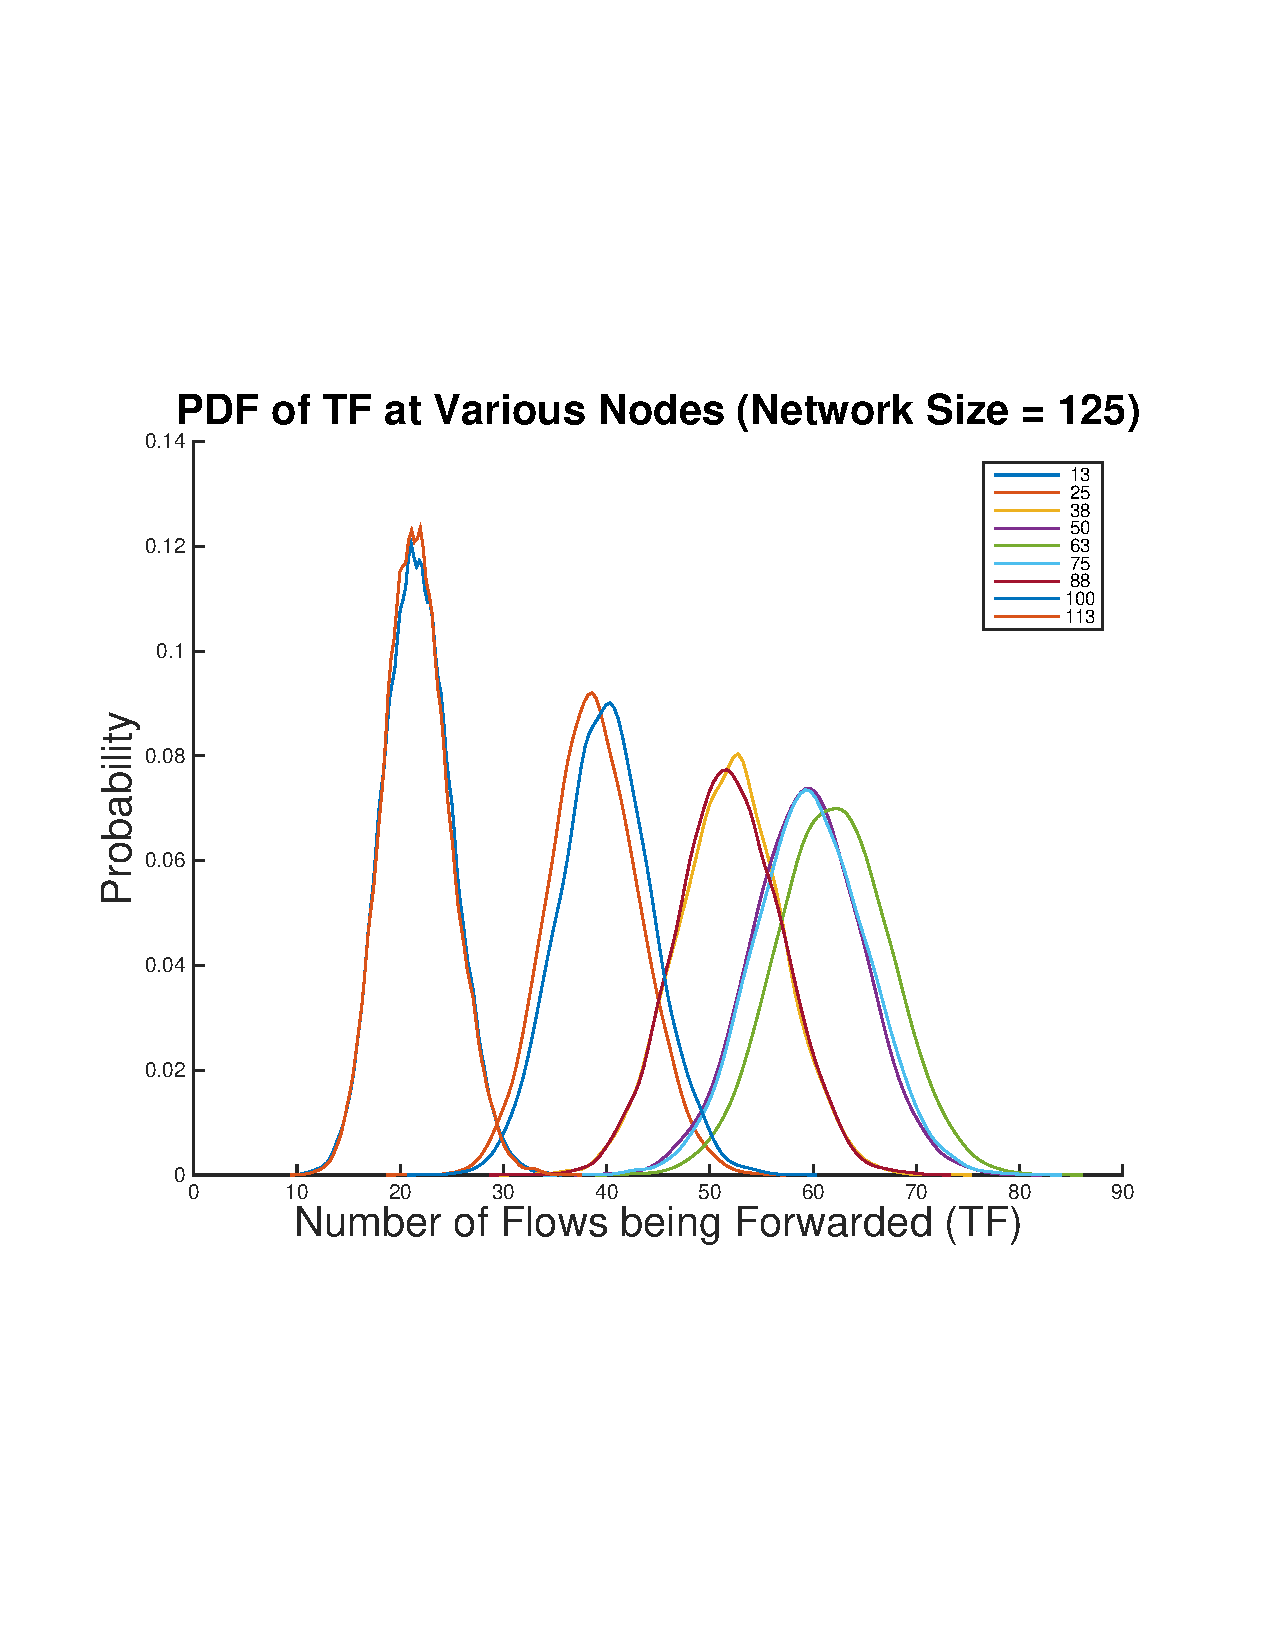
\includegraphics[scale=0.4, clip=true, trim=15mm 65mm 20mm 65mm]{figures/TF_PDFs_line_net_125.pdf}
    \caption{Plotting frequency of experienced Traffic Factors for different node positions in a line network shows that TF is best modeled by a Normal Random Variable. }
    \label{fig:TF_PDFs_line_net}
\end{centering}
\end{figure}

\begin{figure}
\begin{centering}
	\subfigure[The average Traffic Factor for each node of a line network.]{
    		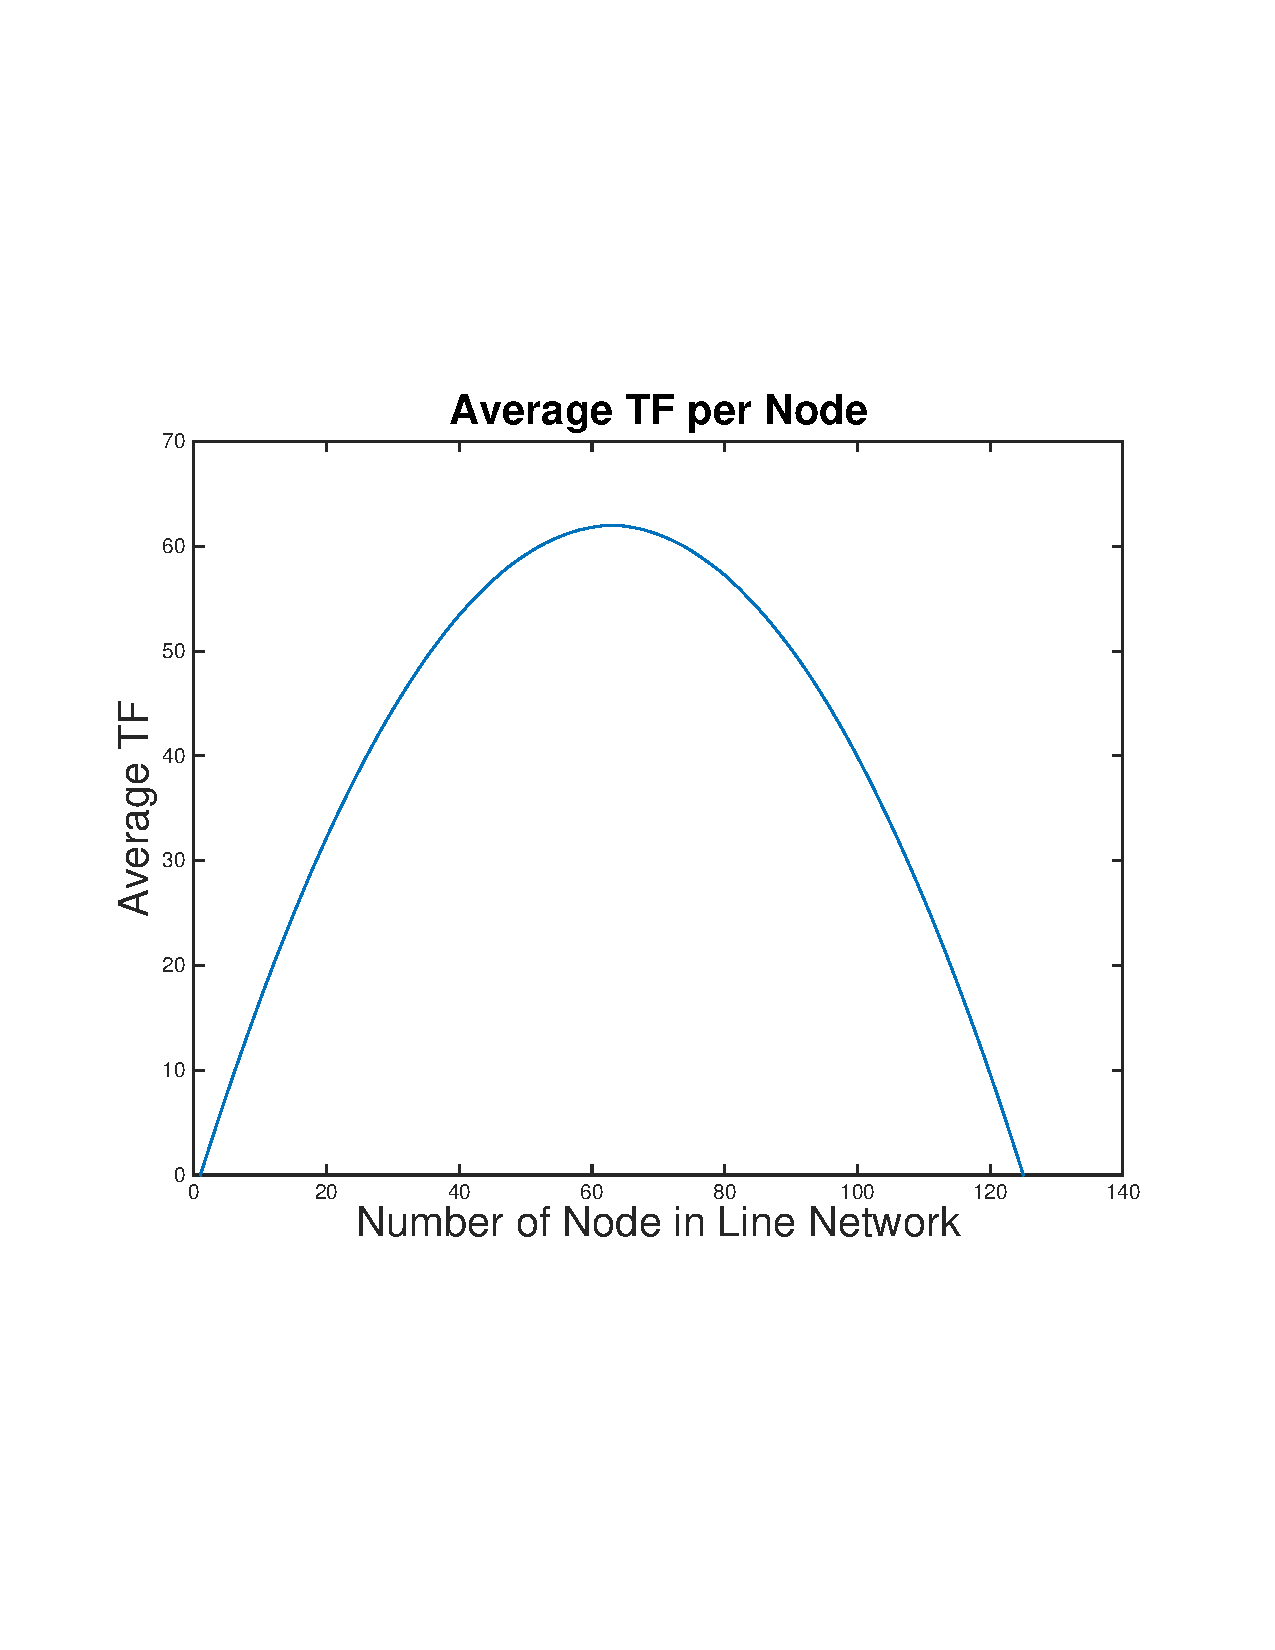
\includegraphics[scale=0.4, clip=true, trim=15mm 65mm 20mm 65mm]{figures/mean_TF_each_node_line_net_125.pdf}
		\label{fig:mean_TF_each_node_line_net}
		}	
	\subfigure[The standard deviation of the Traffic Factor for each node of a line network.]{
    		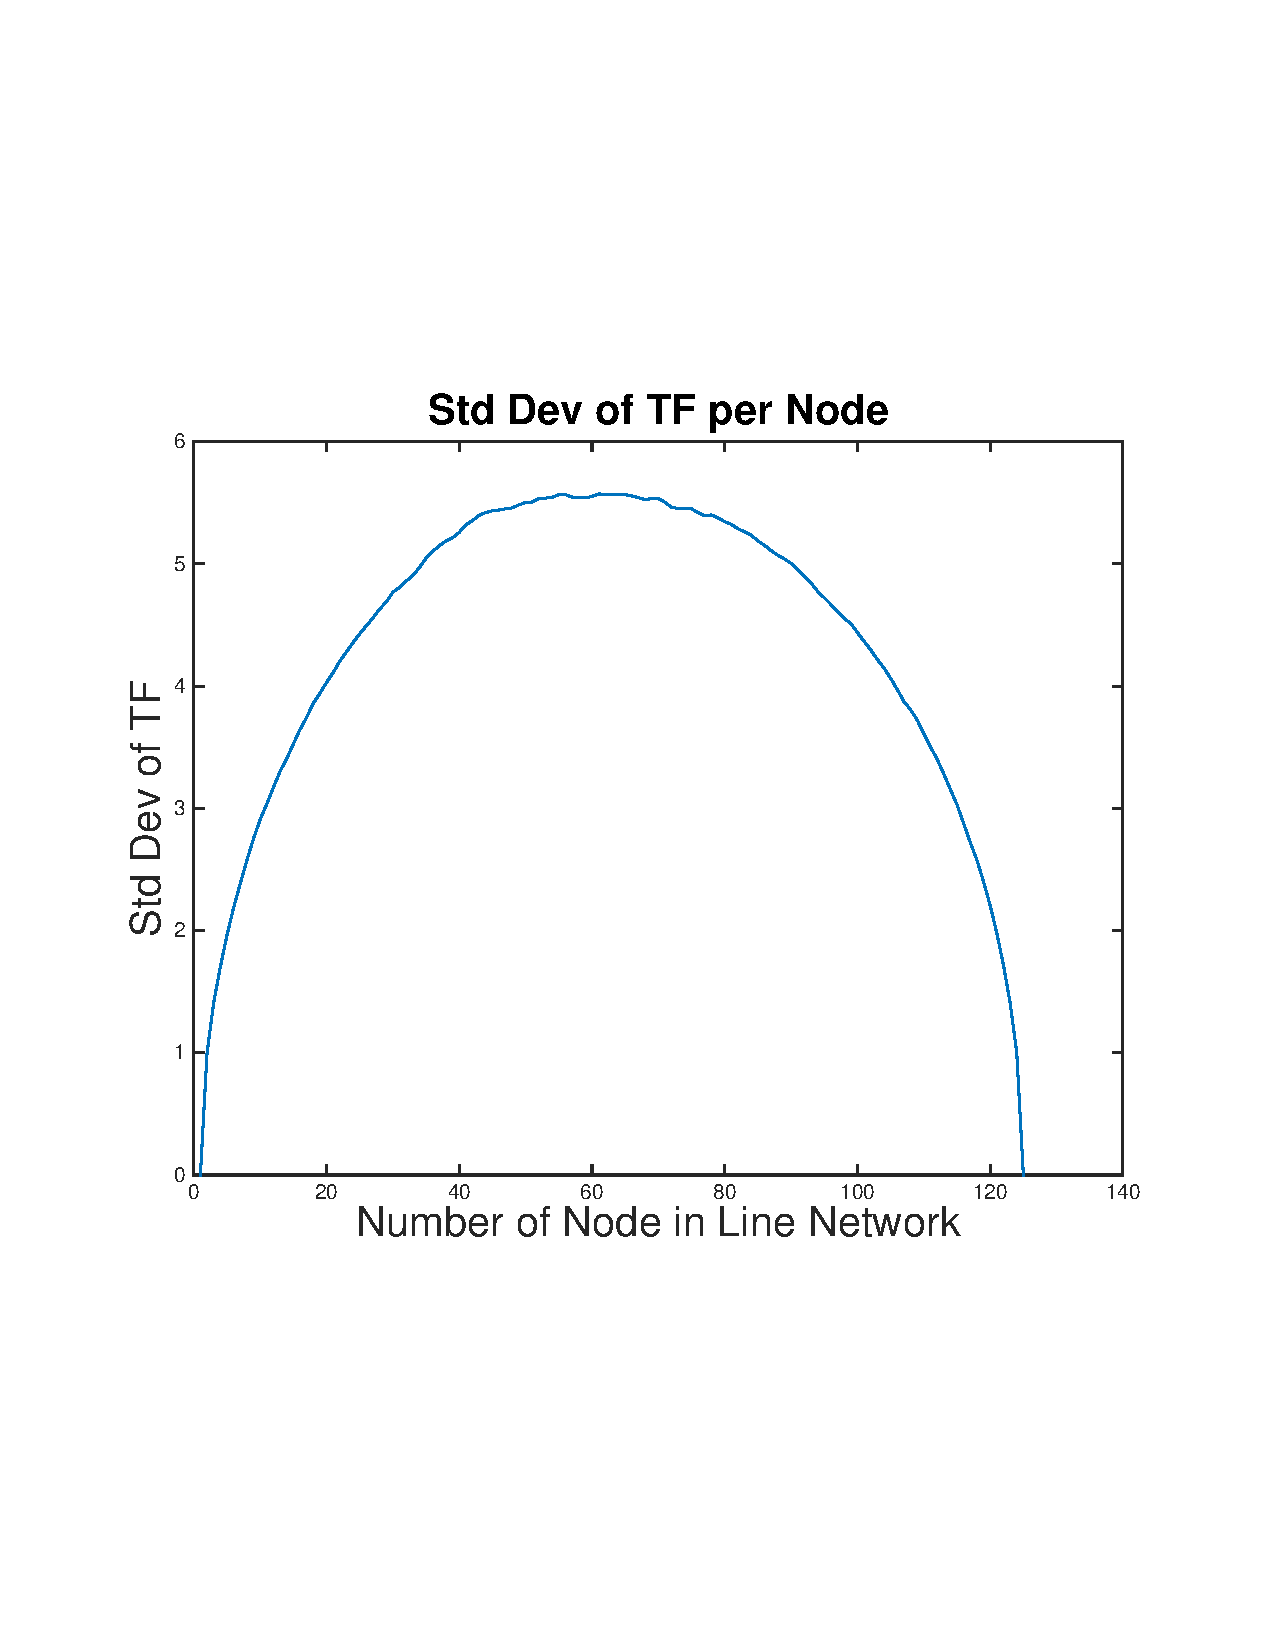
\includegraphics[scale=0.4, clip=true, trim=15mm 65mm 20mm 65mm]{figures/std_dev_TF_each_node_line_net_125.pdf}
		\label{fig:std_dev_TF_each_node_line_net}
		}
	\caption{We can observe the empirical statistical properties of the Traffic Factor for each node's position in a line network (here with 125 nodes).}
	\label{fig:TF_empirical_stats_each_node_line_net}
\end{centering}
\end{figure}

In order to help with modeling the parameters contributing to delay in satisfying queries, we first examine the results of statistics for Traffic Factor from simple simulations implementing the traffic model.  Here, we simply simulated a large number of trials in which destinations were chosen at random for each source and the actual traffic factor and path length statistics were recorded for each node and each trial.  

Figure \ref{fig:TF_PDFs_line_net} shows the empirical PDF of the TF for a sample of the nodes along the line network.  Clearly, the distribution of the TF at each node follows a Normal distribution with varying mean and standard deviation values.  This result is expected and should follow as an application of the Central Limit Theorem (need to define RVs appropriately to make this point more rigorous).  We plot these mean and standard deviation values, also empirically found, for each node in the line network in Figure \ref{fig:TF_empirical_stats_each_node_line_net}.  Using Matlab's curve-fitting tool, we can give an approximate distribution for the Traffic Factor at node $x$, i.e. in $x_{th}$ position from one end, in the network:

\begin{equation}
	f_{TF_x} = \mathcal{N}(-0.016x^2+2x-2, -0.0011x^2+0.138x+1.42)
\end{equation}

Let's call these two functions $\mu_{TF}(x)$ and $\sigma_{TF}(x)$.  For a flow originating at node $i$, we want the PDF of the Traffic Factor.  Let's call the destination of the flow $j$.  Then, let's use $P_{TF}^i$ to represent the PDF of the Traffic Factor for this flow originating at node $i$.  
%First, let's assume a destination node $j$ and define the distribution of TF for this flow, $P_{TF}^{i,j}$.  
We need to first find the node that has the largest expected TF, so we need to find the node $x'$ that has the maximum expected TF:

\begin{equation}
	x' = \argmax_{x = [\min(i,j), \max(i,j)]} \mu_{TF}(x) 
\end{equation}

Then, we can say that the distribution of the TF for this flow would be

\begin{equation}
	f_{TF}^{i}(tf) = \mathcal{N}(\mu(x'), \sigma(x'))
	\label{eq:pdf_TF_1}
\end{equation}

Let's call the randomly chosen destination of the flow $j$. If $i < N/2$, since the maximum of $\mu_{TF}$ is at $N/2$, the value of $x'$ is given by: 

\begin{eqnarray*}
	x' &=&
		\left\{\begin{array}{ll}
		i & \mbox{    } j < i \\
		j & \mbox{    } i < j < \frac{N}{2} \\
		\frac{N}{2} & \mbox{    } \frac{N}{2} \leq j \leq N \\ 
		0 &\mbox{o.w.}
		\end{array}\right.
\end{eqnarray*}

Since $j$ is given  by a uniform random variable, the probability distribution of $x'$ for a flow originating in node $i$ would be

\begin{eqnarray}
	f_{X'}^i(x') &=&
		\left\{\begin{array}{ll}
		\frac{i}{N} & x' = i  \\
		 \frac{1}{2} - \frac{i}{N} & i < x' < \frac{N}{2} \\
		 \frac{1}{2} & x' = \frac{N}{2} \\ 
		0 &\mbox{o.w.}
		\end{array}\right.
		\label{eq:PDF_x_prime}
\end{eqnarray}

Then, the distribution of the PDF for the Traffic Factor of a flow originating in node $i$ is given by Equation (\ref{eq:pdf_TF_1}), where $x'$ is first sampled from the distribution in Equation (\ref{eq:PDF_x_prime}).  This distribution can be fully described with a mixture distribution as follows:

\begin{eqnarray}
\nonumber
	f_{TF}^i (tf) = &&\frac{i}{N} \cdot \mathcal{N}(\mu(i),\sigma(i))  \\ \nonumber
			   &+& \sum\limits_{k=i}^{\frac{N}{2}-1} \cdot \frac{\frac{1}{2}-\frac{i}{N}}{\frac{N}{2} - i}\mathcal{N}(\mu(k),\sigma(k))  \\
			   &+& \frac{1}{2} \cdot \mathcal{N} (\mu(\frac{N}{2}),\sigma(\frac{N}{2}))
\label{eq:full_PDF_TF}
\end{eqnarray}

\begin{figure}
\begin{centering}
    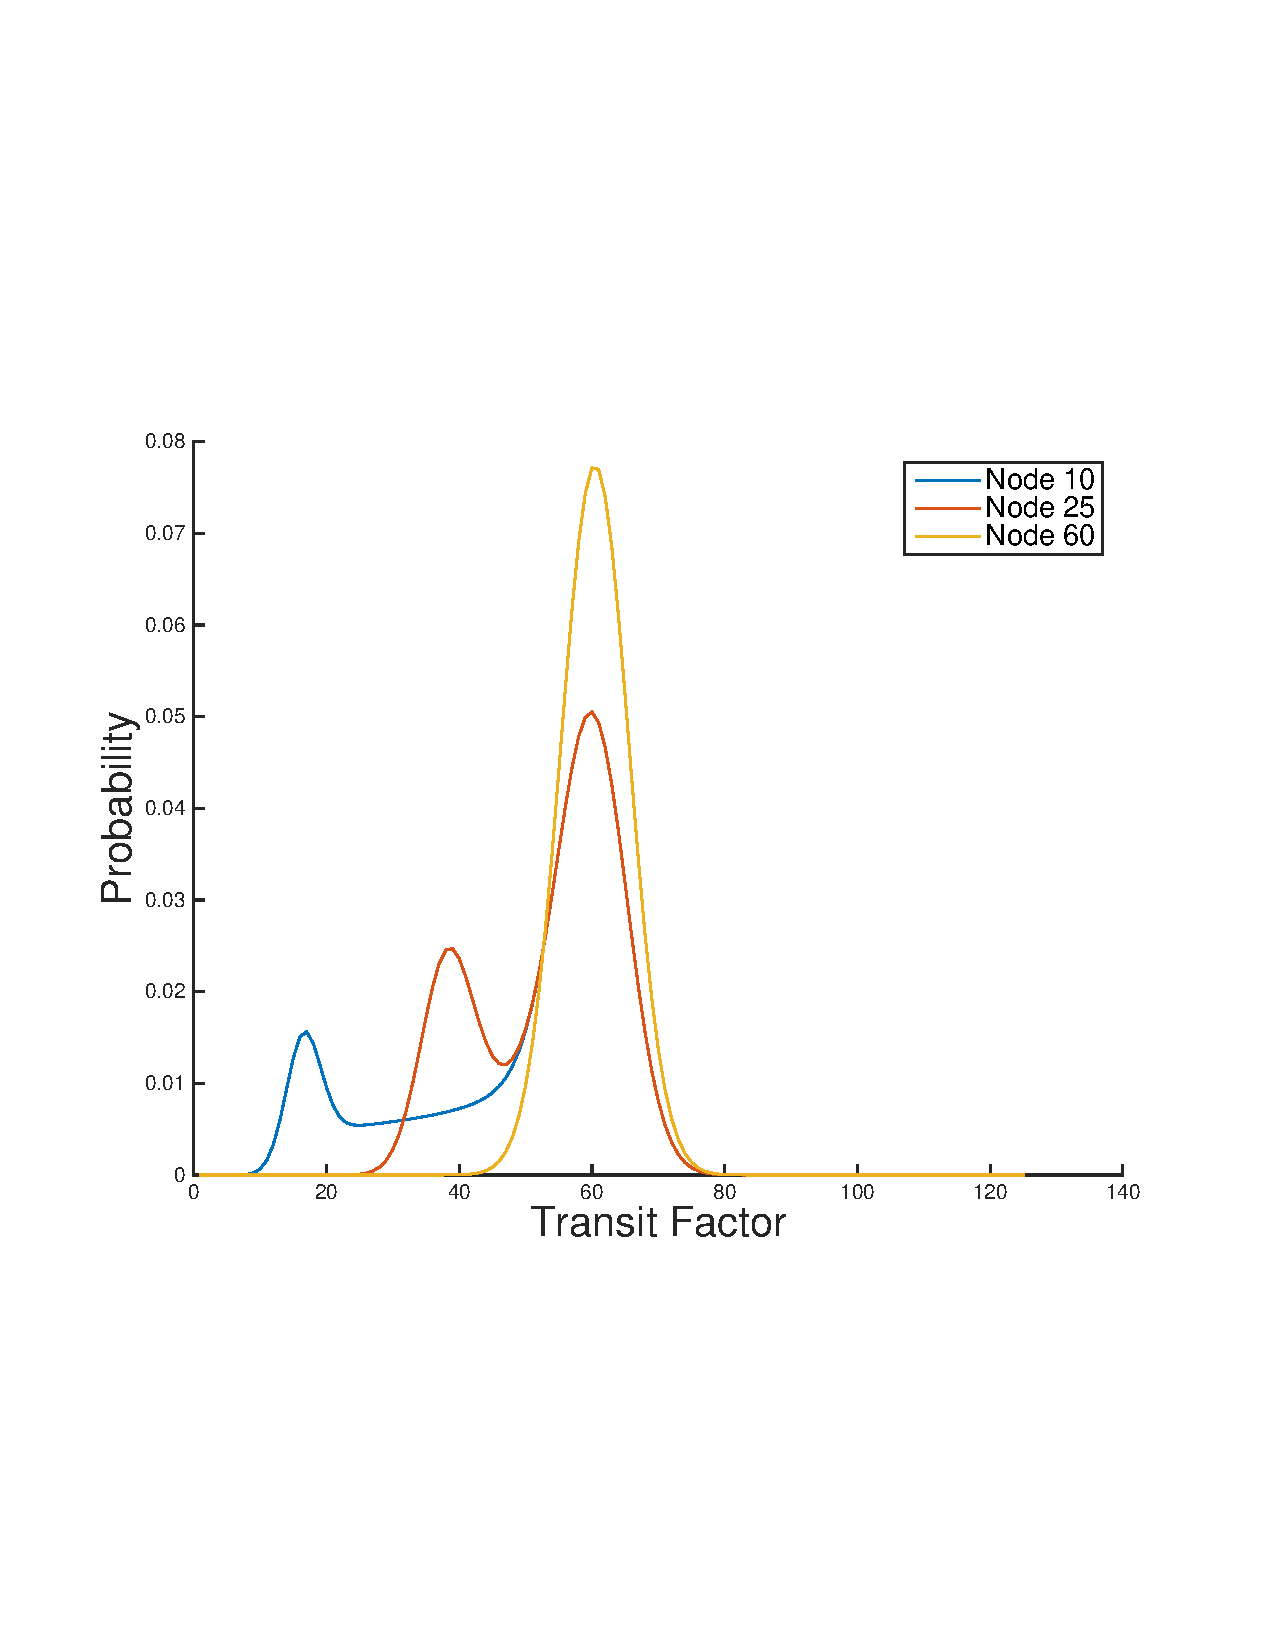
\includegraphics[scale=0.4, clip=true, trim=15mm 65mm 20mm 65mm]{figures/PDF_TF_line_net_125.pdf}
    \caption{PDF of Traffic Factor for flows originating in Nodes 10, 25, and 60 in a 125 node line network.}
    \label{fig:PDF_TF_line_net}
\end{centering}
\end{figure}

\begin{figure}
\begin{centering}
    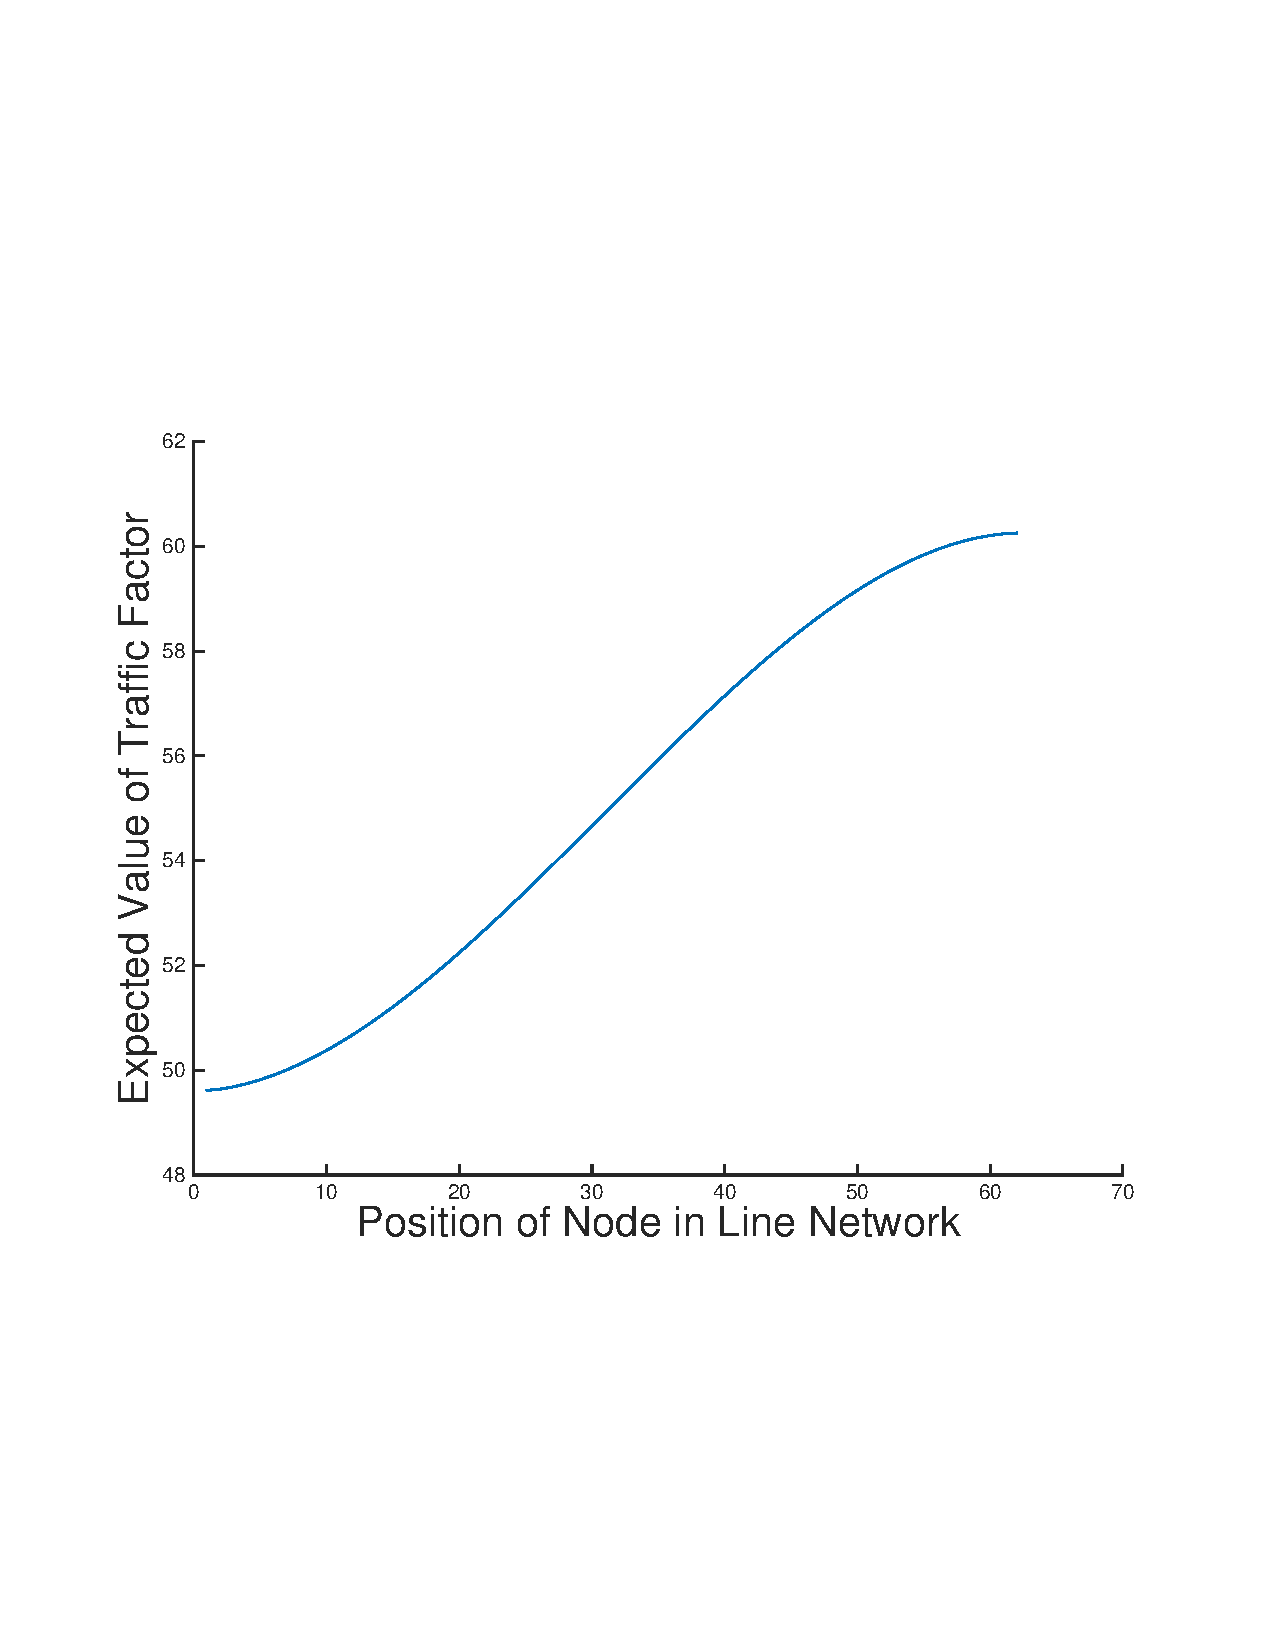
\includegraphics[scale=0.4, clip=true, trim=15mm 65mm 20mm 65mm]{figures/EV_TF_line_net_125.pdf}
    \caption{Expected Value of Traffic Factor for flows originating in Nodes 5-62 in a 125 node line network.}
    \label{fig:EV_TF_line_net}
\end{centering}
\end{figure}

Figure \ref{fig:PDF_TF_line_net} shows the distribution in Equation \ref{eq:full_PDF_TF} for several chosen nodes in a line network.  Figure \ref{fig:EV_TF_line_net} displays the expected value of TF for flows originating in nodes $1$ to $62$ in a $125$ node line network.  

\subsection{Path Length}

\begin{figure}
\begin{centering}
    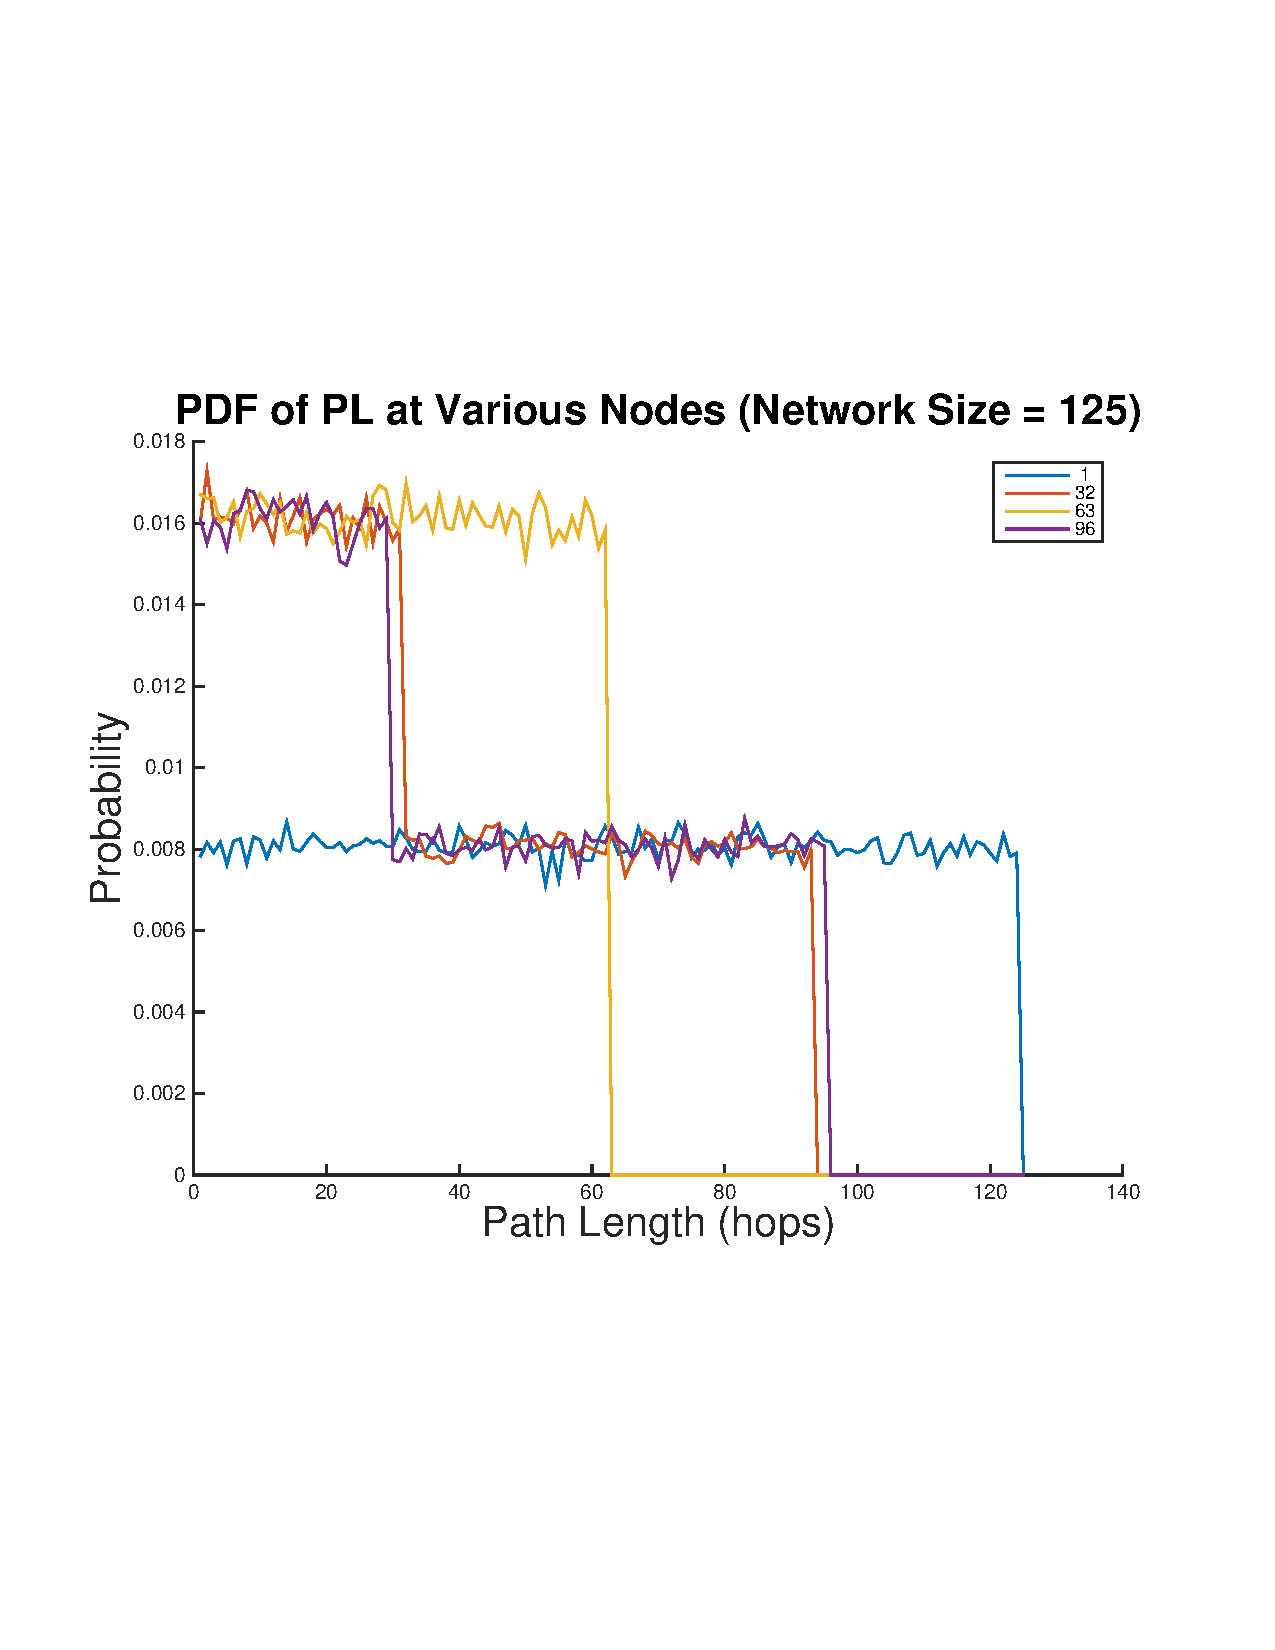
\includegraphics[scale=0.4, clip=true, trim=15mm 65mm 20mm 65mm]{figures/PL_PDFs_each_node_line_net_125.pdf}
    \caption{Plotting the frequency of experienced Path Lengths for different node positions in a line network shows that PL can be modeled as disjoint Uniform Random Variables.}
    \label{fig:PL_PDFs_line_net}
\end{centering}
\end{figure}

Next, we can capture the distribution of the path length given by flows originating in node $i$ of the network.  Since our traffic model is to choose destination nodes with uniform randomness, we can derive the distribution of path lengths for flows with source node $i$ as follows (details can be given if needed).  Again, let us just assume that $i$ is less than $N/2$, since we can use symmetry to draw the same conclusion about nodes greater than $N/2$.

\begin{eqnarray*}
	f_{PL}^i(pl) &=&
		\left\{\begin{array}{ll}
		\frac{2}{N} & \mbox{for } 1 < pl < (i-1) \\
		\frac{1}{N} & \mbox{for } i \leq pl \leq N-i \\
		0 &\mbox{elsewhere}
		\end{array}\right.
\end{eqnarray*}

\begin{figure}
\begin{centering}
    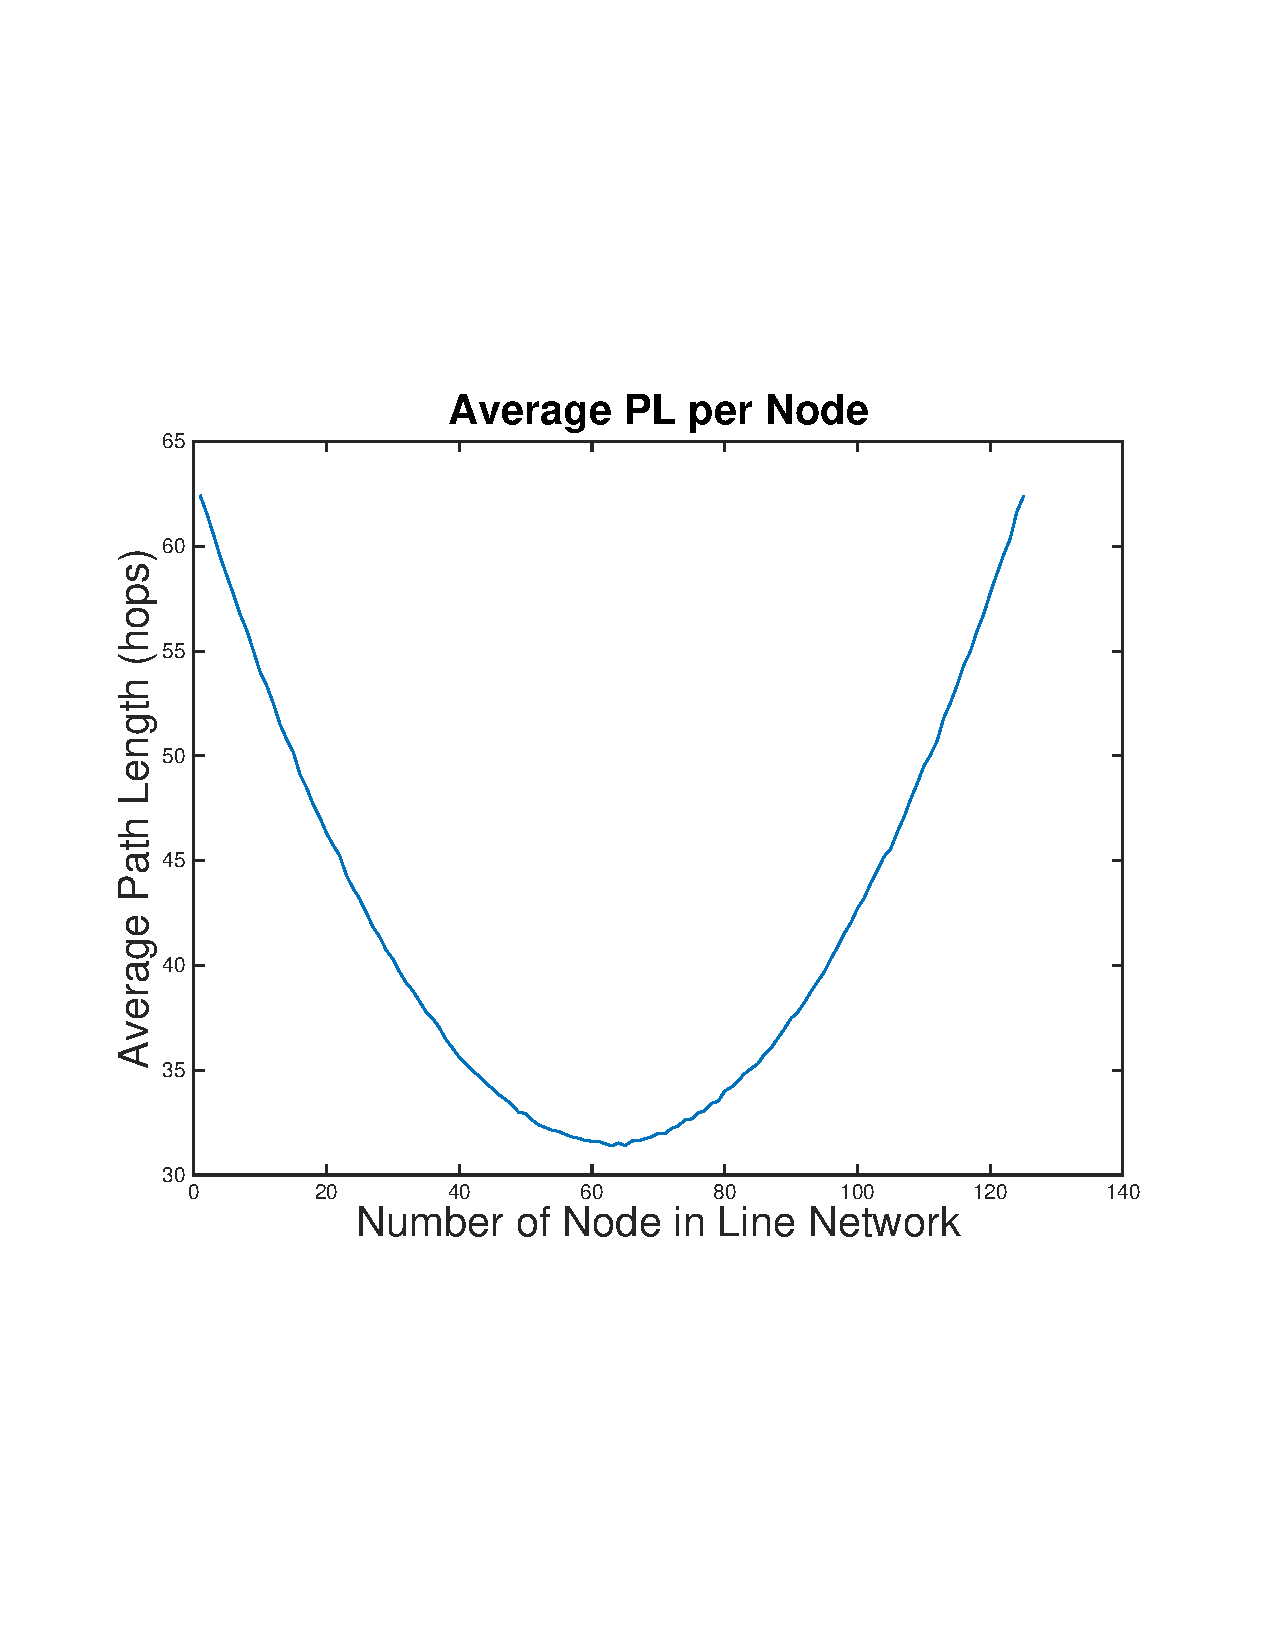
\includegraphics[scale=0.4, clip=true, trim=15mm 65mm 20mm 65mm]{figures/mean_PL_each_node_line_net_125.pdf}
    \caption{The average value of path length intuitively peaks at the edges of the line network and is minimum in the middle.}
    \label{fig:mean_PL_each_node_line_net}
\end{centering}
\end{figure}

While the expected value for the path length is not derived here yet, its empirical value for nodes in each position are shown in Figure \ref{fig:mean_PL_each_node_line_net}.  Not surprisingly, values of mean path length range from $~N/2$ at the end of the network to $~N/2$ in the middle of the network.  



%Is the Delay Factor dependent on node position?  It must be...similar to path length, a node's position affects the probability of choosing a route with or against the flow of scheduling.  
%Finally, we can give a simple expression for the Delay Factor: 
%\begin{eqnarray*}
%	P_{DF_x}(l) &=&
%		\left\{\begin{array}{ll}
%		\frac{2}{N} & \mbox{for } 1 < l < \min(i,N-i) \\
%		\frac{1}{N} & \mbox{for } \min(i,N-i) \leq l \leq \max(i,N-i) \\
%		0 &\mbox{elsewhere}
%		\end{array}\right.
%\end{eqnarray*}


